%%% In this section, you will describe all of the various artifacts that you will generate and maintain during the project life cycle. Describe the purpose of each item below, how the content will be generated, where it will be stored, how often it will be updated, etc. Replace the default text for each section with your own description. Reword this paragraph as appropriate.

\subsection{Major Documentation Deliverables}

\subsubsection{Project Charter}
This document will be maintaned using github and will be often updated when the team needs to change certain implications. The initial version will be delivered by September 2019 and final version will be delivered by December 2019

\subsubsection{System Requirements Specification}
This document will be maintaned using github and will be often updated when the team needs to change certain implications. The initial version will be delivered by September 2019 and final version will be delivered by December 2019

\subsubsection{Architectural Design Specification}
This document will be maintaned using github and will be often updated when the team needs to change certain implications. The initial version will be delivered by September 2019 and final version will be delivered by December 2019

\subsubsection{Detailed Design Specification}
This document will be maintaned using github and will be often updated when the team needs to change certain implications. The initial version will be delivered by September 2019 and final version will be delivered by December 2019

\subsection{Recurring Sprint Items}

\subsubsection{Product Backlog}
Items from the SRS will be added to the product backlog in order of importance. We will make decisions on which items to prioritize with a group vote. GitHub will be used to keep an up-to-date version of the product backlog.

\subsubsection{Sprint Planning}
How will each sprint plan be planned? How many sprints will there be (you need to look at the schedules for this course and previous Senior Design II courses during the appropriate semesters to figure this out).

\subsubsection{Sprint Goal}
The spring goal will decided by the group. We will discuss what a reasonable goal will be based on our knowledge and the difficulty of the task. The input from the customer will also be taken in consideration.

\subsubsection{Sprint Backlog}
The team leader will decided what backlog products will make into the sprint backlog. The backlog will be maintained by the team leader in a shared file in Google Drive or GitHub.


\subsubsection{Task Breakdown}
Each individual from the team will list their programming skills and based on that will be given a task to complete. The amount of time that they have to complete will be documented in the sprint as well, also if they find a task that they think it fits their set of skill, they can claim that task for themselves.

\subsubsection{Sprint Burn Down Charts}
The team captain will generate the burndown chart. GitHub will be able to keep track of who completed which tasks. The burndown chart will be an excel graph that keeps track of how many tasks are remaining.

\begin{figure}[h!]
    \centering
    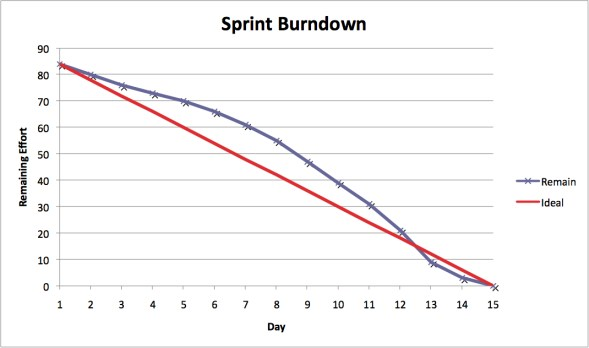
\includegraphics[width=0.5\textwidth]{images/Sprint_Burndown}
    \caption{Example sprint burn down chart}
\end{figure}

\subsubsection{Sprint Retrospective}
The scrum master will meet with the team to discuss what went well and what can be improved on the next sprint. This meeting will happen within a week after each sprint is completed. It will be documented in a sprint retrospective file and turned in December 2019.

\subsubsection{Individual Status Reports}
After each sprint, each team member will report what they have accomplished. It will contain what items were completed, how much money was spent, and any issues that need to be handled.

As a group, we are going to report status of the overall development of the application and reports of the functionality and interface between the application and the RFID scanner.  In addition, every week each individual will need to report their status to every team member in the group, that way everyone is up-to-date in the progress of the application and it's functionality with the RFID scanner.  The key items that'll need to be reported are as follows:
1.) Status of GUI development
2.) Testing of different versions of Android operating systems to make sure the application and the RFID scanner interface correctly.
3.) Reports of beverage information safely stored in the database.
4.) Reports of bugs found in the application and fixes applied to the application.
5.) Reports of the condition of the RFID scanner throughout development and testing.

\subsubsection{Engineering Notebooks}
The engineering notebooks will be updated after each team meeting which will happen, at a minimum, every two weeks. During the two week interval, at least one page of documentation will be completed. Each member will keep track of their on work in their own ENB. At least one other teammate will sign as a witness another teammate in their ENB.


\subsection{Closeout Materials}

\subsubsection{System Prototype}
The system prototype will include a mobile app, an RFID reader, possibly an RFID tag printer, and a database. It will be demonstrated upon completion for the class in December 2019. There will be no Prototype Acceptance Test (PAT) with the customer. Nothing will be demonstrated off-site.

\subsubsection{Project Poster}
The poster will include the product name, team name, team vision, product picture, and key features of the product. It will be presented during the product presentation in December 2019.

\subsubsection{Web Page}
The product web page will include a shop to sell the product and describe the features of the product. In addition, it will describe how the product was designed and why the product was designed. It will be accessible to the public. This will be delivered December 2019. The web page will be completed at closeout.

\subsubsection{Demo Video}
The demo video will include a brief demonstration of the computer screen and smart phone applications working together as well one of our members working with the scanner and label maker. The approximated time will be about 2 - 4 minutes. The topics covered will be the label making, scanning a new product, managing the database from the desktop application.

\subsubsection{Source Code}
The source code will be maintained in GitHub. Both the source code and the executable files will be provided to the customer. All of there will be saved in a cloud service so that it can be downloaded as many times is needed. The source code will be posted in a public repository in GitHub for the general public with a MIT license. The license will be listed in the "read-me" file or its own file.

\subsubsection{Source Code Documentation}
The specific documentation standard will be decided at a later date. We will use Doxygen to document the product. The final documentation will be available in PDF form and HTML form on the product web page.

\subsubsection{Hardware Schematics}
The project is only software.

\subsubsection{CAD files}
The project is only software.

\subsubsection{Installation Scripts}
The mobile application will be sent through GitHub and installed in the device via Android Studio. If any desktop application is developed, it will be provided using a installation script. 

\subsubsection{User Manual}
The customer will be provided with a digital manual and there will also be instructions in the application as well. If the software proves to be more complicated that we think, then a setup video will be created to show the customer how to operate the software and hardware.
